\documentclass[11pt,a4paper]{article}
\usepackage{extarrows}
\usepackage[sort]{natbib}
\usepackage{fancyhdr}
\usepackage{graphicx}
\usepackage{amsmath,amsfonts,amsthm,nicefrac,latexsym,amsfonts,amsbsy,bm}
\usepackage[nottoc,numbib]{tocbibind}
\usepackage{lipsum}

%-----------------------------------------------------------------------------------USER INTRODUCED PACKAGES BEGINS
\usepackage{amsmath,amsthm}
\usepackage{mathtools}
\usepackage{titlesec}
\usepackage{hyperref} 
\usepackage{graphicx}
\usepackage{float}
\usepackage{amssymb}
\usepackage{amscd}
\usepackage{bm}
\usepackage{extarrows}
\usepackage{appendix}
\usepackage{subcaption}
\usepackage{listings}
\usepackage{color}

\definecolor{dkgreen}{rgb}{0,0.6,0}
\definecolor{gray}{rgb}{0.5,0.5,0.5}
\definecolor{mauve}{rgb}{0.58,0,0.82}

\lstset{frame=tb,
	language=Matlab,
	aboveskip=3mm,
	belowskip=3mm,
	showstringspaces=false,
	columns=flexible,
	basicstyle={\small\ttfamily},
	numbers=none,
	numberstyle=\tiny\color{gray},
	keywordstyle=\color{blue},
	commentstyle=\color{dkgreen},
	stringstyle=\color{mauve},
	breaklines=true,
	breakatwhitespace=true,
	tabsize=3
}
%-----------------------------------------------------------------------------------USER INTRODUCED PACKAGES ENDS


%----- you must not change this -----------------
\oddsidemargin 0.2cm
\topmargin -1.0cm
\textheight 24.0cm
\textwidth 15.25cm
\parindent=0pt
\parskip 1ex
\renewcommand{\baselinestretch}{1.1}


\pagestyle{fancy}
\pagenumbering{arabic}
%----------------------------------------------------



%---- please enter 
\def\StudentName{Zhaozhi Liu}			% insert here your name
\def\StudentNumber{s2058599}			% insert here your student number
%\def\Proposer{Dr Patrick Ilg}		% insert here name of proposer

%-----------------------------------------------------------------------------------USER DEFINED COMMANDS/ENVIRONMENTS BEGINS



\newtheorem{theorem}{Theorem}[section]
\newtheorem{defn}{Definition}[section]
\newtheorem{lemma}{Lemma}
\newtheorem{proposition}{Proposition}
\newtheorem{coro}{Corollary}
\newtheorem*{lem}{Lemma}
%-----------------------------------------------------------------------------------USER DEFINED COMMANDS/ENVIRONMENTS ENDS




%-----------------------------------------------------------------------------------HEADER AND TITLE INFORMATION BEGINS



%----- you must not change this -----------------
\lhead{\normalsize \textrm{Assignment 2}}
\chead{}
\rhead{\normalsize \StudentNumber}
\lfoot{\normalsize \textrm{MATH11158}}
\cfoot{\thepage}
%\rfoot{\Proposer}
\setlength{\fboxrule}{4pt}\setlength{\fboxsep}{2ex}
\renewcommand{\headrulewidth}{0.4pt}
\renewcommand{\footrulewidth}{0.4pt}
\setlength{\headheight}{15pt} 

%----------------------------------------------------





\title{Optimization Methods in Finance \\ Assignment 2}
\author{\StudentName\\ \StudentNumber \\ \phantom{} \\ University of Edinburgh }



%-----------------------------------------------------------------------------------HEADER AND TITLE INFORMATION ENDS
\date{}
\begin{document}
\maketitle
\section*{Part 1 }
\section*{Question 1}
\textbf{Sol:}\\
\textbf{(1)}:
We first prove the following lemma:
\begin{lem}
	\textit{When minimising a concave function over a compact convex set, there exists at
		least one extreme point of the set that is an optimal solution}
\end{lem}
In this question since we assume that $Y$ is a convex polytope and the optimization problem is considered over the set $Y$, it is sufficient for us to prove the following:
\begin{lem}
	\textit{When minimising a concave function over a convex polytope, there exists at
least one extreme point of the polytope that is an optimal solution}
\end{lem}
Suppose $\lambda \in \mathbb{R}_{+}^{K}$ and $\sum_{i=1}^{K}\lambda_{i}=1$, since $Y$ is a convex polytope with extreme point $\left\{\bar{y}^{1}, \ldots, \bar{y}^{K}\right\}$, for any $y\in Y$, we have the convex combination $y=\lambda^{T}\bar{y}$ for some $\lambda$, suppose $h$ is a concave function over $Y$ therefore,
$$\begin{aligned}h(y) = h(\lambda^{T}\bar{y})&=h(\lambda_{1}\bar{y}^{1}+ \ldots+\lambda_{K}\bar{y}^{K})\\
&\geq \lambda_{1}h(\bar{y}^{1})+\ldots+\lambda_{K}h(\bar{y}^{K})\\
&\geq \inf_{i = 1,\ldots,K}h(\bar{y}^{i})
\end{aligned}$$
Which means $h$ attains the minimum at least one extreme point of the polytope $Y$.
Then we prove the first part of the question. We now turn to the main problem of Question (1).
$$\begin{array}{ll}
\underset{y\in Y}{\operatorname{minimize}} 
& f_{0}(y,\omega) \\ \text { subject to }
& f_{i}(y,\omega)+g_{i}(x,\omega)-h_{i}(\omega)\leq0, \quad i=1,2, \ldots, m. \ y\in Y \\ 
\end{array}$$
The associate Lagrangian is 
$$\mathcal{L}(x,y,\omega)=f_{0}(y,\omega)+\sum_{i=1}^{m}\lambda_{i}(f_{i}(y,\omega)+g_{i}(x,\omega)-h_{i}(\omega))$$
For $\lambda\geq \textbf{0},\ \forall y\in Y $.
Due to the constraints we have that $f_{0}$ is bounded below by $\mathcal{L}(x,y,\omega)$.
$$f_{0}(y,\omega)\geq\mathcal{L}(x,y,\omega)$$ The Lagrange dual function is 
$$\nu(\lambda)=\min_{y\in Y}\mathcal{L}(x,y,\omega)$$
Then we have $$f_{0}(y,\omega)\geq\nu(\lambda)$$
By taking minimization for $y$ on the left side, we have $$Q(x,\omega)\geq\nu(\lambda)$$
Since $\nu(\lambda)$ is a concave function for $y\in Y$, by the lemma, we have 
$$Q(x,\omega)\geq -h^{T}(\omega)\lambda + \sum_{i=1}^{m}\lambda_{i}g_{i}(x,\omega)+\min_{k=1,\ldots,K}\left[f_{0}(\bar{y}^{k},\omega)+\sum_{i=1}^{m}\lambda_{i}f_{i}(\bar{y}^{k},\omega)\right]$$
(2): Consider $x_{1},x_{2}$ with corresponding recourse $y_{1},y_{2}$, which are optimal for $x_{1}$ and $x_{2}$.
We have $y(\lambda)=\lambda y_{1}+(1-\lambda)y_{2}, \ \lambda\in[0,1]$.
Therefore, since $f_{i}$ is convex, and from the constraints of the optimal problem, we have the following. $$\begin{aligned}
f_{i}(y(\lambda),\omega)&=f_{i}(\lambda y_{1}+(1-\lambda)y_{2},\omega)\\
&\leq \lambda f_{i}(y_{1},\omega)+(1-\lambda)f_{i}(y_{2},\omega)\\
&\leq \lambda\left[h_{i}(\omega)-g_{i}(x_{1},\omega)\right]+(1-\lambda)\left[h_{i}(\omega)-g_{i}(x_{2},\omega)\right]\\
&= h_{i}(\omega)-\left[\lambda g_{i}(x_{1},\omega)+(1-\lambda)g_{i}(x_{2},\omega)\right]\\
\text{Due to convexity of $g$}\\
& \leq h_{i}(\omega)-g_{i}(\lambda x_{1}+(1-\lambda)x_{2},\omega)\\
& = h_{i}(\omega)-g_{i}(x(\lambda),\omega) \quad \because y(\lambda) \ \text{is feasible for $x(\lambda)$}
\end{aligned}$$
Then there is $$\begin{aligned}
Q(x(\lambda),\omega)\leq f_{0}(y(\lambda),\omega)&\leq f_{0}(y(\lambda),\omega)\\
&= f_{0}(\lambda y_{1}+(1-\lambda)y_{2},\omega)\\
&\leq \lambda f_{0}(y_{1},\omega)+(1-\lambda)f_{0}(y_{2},\omega)\\
&= \lambda Q(x_{1},\omega)+(1-\lambda)Q(x_{2},\omega)
\end{aligned}$$
(3):
By letting $f_{0}(y,\omega)=q(\omega)^{T}y$, $f(y,\omega)=W(\omega)y$, $g(x,\omega)=T(\omega)x$, we have that $f_{0},f,g$ are all convex function, then by (2), we have that $Q(X,\omega)$ is convex. 
\section*{Question 2}
\textbf{Sol:}\\
(1): From the definition of $\mathcal{PSD}_{n}$ and $\mathcal{COP}_{n}$, the difference is that the vector $\textbf{v}$ is non-negative in $\mathcal{COP}_{n}$\\
(2):\\ $\mathcal{DNN}_{n}$: \\
For $\forall A \text{ in } \mathcal{DNN}_{n}$, we have for any $\lambda>0$, there is $\lambda A\geq 0,\ (\lambda A)^{T}=\lambda A^{T}=\lambda A$, then we have $\lambda A\in \mathcal{S}^{+}_{n}$. For any $v$, there is $$v^{T}\lambda Av = \lambda(v^{T}Av)\geq 0$$
Then we have $\lambda A\in \mathcal{PSD}_{n}$, therefore $\lambda A \in \mathcal{PSD}_{n}\cap\mathcal{S}^{+}_{n}=:\mathcal{DNN}_{n}$. Hence, $\mathcal{DNN}_{n}$ is a cone.\\
For any $A,B\in \mathcal{DNN}_{n}$, $A+B\geq0,\ (A+B)^{T}=A^{T}+B^{T}=A+B\in \mathcal{S}_{n}^{+}$.\\
For any $v$, there is $$v^{T}(A+B)v=v^{T}Av+v^{T}Bv\geq 0$$ Hence $A+B\in \mathcal{PSD}_{n}\cap\mathcal{S}^{+}_{n}=:\mathcal{DNN}_{n}$.\\ \\ 
$\mathcal{COP}_{n}$:\\
For $\forall \lambda>0,\ A \in \mathcal{COP}_{n}$, we have $\lambda A\geq 0,\ (\lambda A)^{T}=\lambda A^{T}=\lambda A$, then we have $\lambda A\in \mathcal{S}_{n}$. For any non-negative $v$, we have $$v^{T}(\lambda A)v=\lambda (v^{T}Av)\geq0$$Therefore $\lambda A\in \mathcal{COP}_{n}$, $\mathcal{COP}_{n}$ is a cone.
For any $A,B\in \mathcal{COP}_{n}$, $A+B\geq0,\ (A+B)^{T}=A^{T}+B^{T}=A+B\in \mathcal{S}_{n}$. And we have $$v^{T}(A+B)v=v^{T}Av+v^{T}Bv\geq 0$$
Hence $A+B\in \mathcal{COP}_{n}$. $\mathcal{COP}_{n}$ is a cone.\\ \\
$\mathcal{CP}_{n}$:\\
Similar as before, for any $\lambda>0$, and any $A \in \mathcal{CP}_{n}$. Obviously, $\lambda A\in \mathcal{S}_{n}$. We have $$\lambda A = \lambda (BB^{T})=(\sqrt{\lambda}B)(\sqrt{\lambda}B)^{T}$$ For some $B \geq \mathbf{0}$. Therefore, $\mathcal{CP}_{n}$ is a cone.\\
(3): We let
$$\mathcal{C P}_{n} \underset{\textcircled{1}}{\subseteq} \mathcal{D} \mathcal{N} \mathcal{N}_{n} \underset{\textcircled{2}}{\subseteq} \mathcal{P} \mathcal{S} \mathcal{D}_{n} \underset{\textcircled{3}}{\subseteq} \mathcal{P} \mathcal{S} \mathcal{D}_{n}+\mathcal{S}_{n}^{+} \underset{\textcircled{4}}{\subseteq} \mathcal{C O P}_{n} \underset{\textcircled{5}}{\subseteq} \mathcal{C} \mathcal{P}_{n}^{*}$$
$\textcircled{1}$: For $\forall$ matrix $A\in\mathcal{CP}_{n}$, and $\forall$ vector $v$, we have $A=B B^{T}\geq\mathbf{0}$ for some $B \geq \mathbf{0}$, and hence $A\in\mathcal{S}_{n}^{+}$. We also have $$v^{T}Av=v^{T}(BB^{T})v=(v^{T}B)(B^{T}v)=(v^{T}B)(v^{T}B)^{T}\geq0$$Therefore, $A\in\mathcal{PSD}_{n}\cap \mathcal{S}_{n}^{+}=:\mathcal{DNN}_{n}\Rightarrow$ $\mathcal{C} \mathcal{P}_{n} \subseteq \mathcal{D} \mathcal{N} \mathcal{N}_{n}$\\ \\ 
$\textcircled{2}$: Obviously, since $\mathcal{D} \mathcal{N} \mathcal{N}_{n}:=\mathcal{P} \mathcal{S} \mathcal{D}_{n} \cap \mathcal{S}_{n}^{+}$, we must have $\mathcal{D} \mathcal{N} \mathcal{N}_{n} \subseteq \mathcal{P} \mathcal{S} \mathcal{D}_{n}.$\\ \\
$\textcircled{3}$: For $\forall$ matrix $A\in \mathcal{PSD}_{n}$, $A=A+\mathbf{0}\in \mathcal{P S D}_{n}+\mathcal{S}_{n}^{+}$, then we have $\mathcal{P S} \mathcal{D}_{n} \subseteq \mathcal{P} \mathcal{S} \mathcal{D}_{n}+\mathcal{S}_{n}^{+}$.\\ \\
$\textcircled{4}$: For $\forall A\in\mathcal{P S D}_{n},\ \forall B\in\mathcal{S}_{n}^{+}$, we have $A+B\in \mathcal{S}_{n}$, and for any non-negative vector $v$, there is $$v^{T}(A+B)v=\underbrace{v^{T}Av}_{\geq 0}+\underbrace{v^{T}Bv}_{\geq0}\geq0$$
Hence, $A+B\in \mathcal{C O P}_{n}\Rightarrow$ $\mathcal{P S D}_{n}+\mathcal{S}_{n}^{+} \subseteq \mathcal{C O P}_{n}$.\\ \\
$\textcircled{5}$:We first write $\mathcal{C} \mathcal{P}_{n}^{*}$
$$\mathcal{C} \mathcal{P}_{n}^{*}:=\left\{  A\in \mathbb{R}^{n \times n} : A \bullet B\geq 0, \forall B\in \mathcal{C P}_{n}  \right\}$$
For $\forall A\in \mathcal{C O P}_{n}$, we need to prove $A\in\mathcal{C P}^{*}_{n}$, which means we should prove $$A \bullet B\geq 0, \forall B\in \mathcal{C P}_{n} $$ Since we have the fact that Frobenius inner product and be written as $$A\bullet B = \mathrm{tr}(A^{T}B)$$
Where tr($\cdot$) denote trace of matrix. Hence we have 
$$\begin{aligned}
A\bullet B &= \sum_{i,j}A_{ij}B_{ij}\\ &=\mathrm{tr}(A^{T}B)\\
&=\mathrm{tr}(A^{T}\sum_{i=1}^{k}x_{i}x_{i}^{T}) \quad x_{i}\text{ is column vector with length }n \\
&=\sum_{i=1}^{k}\mathrm{tr}(A^{T}x_{i}x_{i}^{T})\\
\text{We have the fact that $x^{T}Ax=A\bullet xx^{T}=\mathrm{tr}(A^{T}xx^{T})$}\\
&\xlongequal{A^{T}=A}\sum_{i=1}^{k}x_{i}^{T}Ax_{i}\geq0
\end{aligned}$$
Therefore, we have proved $$A \bullet B\geq 0, \forall B\in \mathcal{C P}_{n} $$ Which implies that $\mathcal{C O P}_{n} \subseteq \mathcal{C} \mathcal{P}_{n}^{*}$\\
(4): Due to the relationship from (3), and we are considering a maximization problem, we have the following relationship. 
$$z_{cop}\geq z_{psd} \geq z_{dnn} \geq z_{cp}$$
The original problem can be written as 
$$
\begin{array}{c}
z^{*}=\max_{x}\mu^{T}x \\
\text { s.t. }
\quad\left(\begin{array}{cc}
0 & \frac{1}{2} f_{i}^{T} \\
\frac{1}{2} f_{i} & Q_{i}
\end{array}\right) \bullet\left(\begin{array}{cc}
1 & x^{T} \\
x & X
\end{array}\right) \leq b_{i} \quad \forall i \\
X=x x^{T}, \ x\in F
\end{array}
$$
For the constraints $X=x x^{T}$, which can be relaxed to $
\left(\begin{array}{cc}
1 & x^{T} \\
x & X
\end{array}\right) \in \mathcal{P} \mathcal{S} \mathcal{D}_{n}
$
Therefore we can get $$z_{psd}\geq z^{*}$$
Furthermore, since we do not allow short-selling, we must have $x$ is non-negative, and hence the constraints become $
\left(\begin{array}{cc}
1 & x^{T} \\
x & X
\end{array}\right) \in \mathcal{C} \mathcal{P}_{n}
$
Thus, the final relation is the following: 
$$z_{cop}\geq z_{psd} \geq z_{dnn} \geq z_{cp}\geq z^{*}$$
\section*{Part 2}
\section*{Question 3}
(1): I used Python batch the data, please see the code in Appendix.\\
(2): I used MATLAB calculate the statistics, please see the code in Appendix.\\
(3): Please see the code in Appendix.
\section*{Question 4}
\textbf{In (1) and (2), we discuss how to determine the gradient in the algorithm, the complete code of the algorithm can be seen in Appendix.}\\
(1): In the step 2 of the algorithm, we do not use the cvx to solve the recourse function. Alternatively, we solve the dual problem: 
$$
\max _{u} \sum_{t=1}^{T}\left(R_{t}-\sum_{i=1}^{n} r_{i, t}(\omega) x_{i}\right) u_{t} \text { s.t. } 0 \leq u_{t} \leq b_{t},\  \forall t
$$
Obviously we can conclude the following: $$
u_{t}^{*}=\left\{\begin{array}{ll}
b_{t}, & \text { if } R_{t}-\sum_{i=1}^{n} r_{i, t}(\omega) x_{i} \geq 0 \\
0, & \text { otherwise }
\end{array} \quad \forall t\right.
$$
Then we can calculate gradient(in the $j^{\text{th}}$-loop):
$$
\frac{\partial }{\partial x_{i}}Q(x_{i},\omega_{k})=-\left[r_{i,1}(\omega_{k}) \ r_{i,2}(\omega_{k}) \ r_{i,3}(\omega_{k})\ r_{i,4}(\omega_{k}) \right]\cdot u^{*}
$$

$$
\frac{\partial z}{\partial x_{i}}=c_{i}+\frac{\partial Q}{\partial x_{i}}
$$
where $i=\{1,2,\ldots,8\},\ k=\{1,2,3,4,5,6,7\}$. $R_{t}$ is the target return for quarter $t$. $\mathbf{r}_{i,t}(\omega_{k})$ is the return rate matrix for $i^{\text{th}}$-index, quarter $t$, scenario $k$. $x$ is our portfolio and $b$ is shortfall penalty costs. $c$ is the expense ratio.\\
(2): In the step 2 of the algorithm, we do not use cvx to solve the recourse problem. The recourse problem is:
$$
Q(x, \omega)=\min _{y} \sum_{t=1}^{T} b_{t} y_{t}(\omega) \text { s.t. } \sum_{i=1}^{n} r_{i, t}(\omega) x_{i}+y_{t}(\omega) \geq R_{t}, t=1, \ldots, T,\ y_{t}(\omega) \geq 0,\ \forall t
$$
For $t=1,2,3,4$, and the $k^{\text{th}}$-scenario $\omega_{k}$ we must have the following:
$$y^{*}_{t}=\max\{0,R_{t}-\textbf{r}_{i,t}(\omega_{k})\cdot x\}=\left[R_{t}-\textbf{r}_{i,t}(\omega_{k})\cdot x\right]^{+}$$
Where $y^{*}$ denote the optimal value for the recourse problem. If we let:
$$
b_{t}^{*}=\left\{\begin{array}{ll}
	b_{t}, & \text { if }y_{t}^{*} > 0 \\
	0, & \text { if }y_{t}^{*} = 0
\end{array} \quad \forall t\right.
$$
The stochastic gradient of scenario $\omega_{k}$ is:
$$g_{k}=-\left[b^{*}_{1}\ b^{*}_{2}\ b^{*}_{3}\ b^{*}_{4}\right]\cdot\left[\begin{array}{c}
\textbf{r}_{i,1}(\omega_{k}) \\
\textbf{r}_{i,2}(\omega_{k}) \\
\textbf{r}_{i,3}(\omega_{k}) \\ 
\textbf{r}_{i,4}(\omega_{k})\\
\end{array}\right]$$
Since we have $7$ scenarios, the gradient is(in the $j^{\text{th}}$-loop) $$\widetilde{g}=\dfrac{1}{7}\sum_{k=1}^{7}g_{k}$$
(3): Denote $K$ be the number of different scenarios, then for the optimal portfolio $x^{*}$, the cost $z(x^{*})$ is:
$$z(x^{*})=c^{T}\cdot x^{*}+\dfrac{1}{K}\sum_{k=1}^{K}\left[b_{1}\ b_{2}\ b_{3}\ b_{4} \right]^{T}\cdot \left[\begin{array}{c}
\left[R_{1}-\textbf{r}_{i,1}(\omega_{k})\cdot x^{*}\right]^{+} \\
\left[R_{2}-\textbf{r}_{i,2}(\omega_{k})\cdot x^{*}\right]^{+} \\
\left[R_{3}-\textbf{r}_{i,3}(\omega_{k})\cdot x^{*}\right]^{+} \\ 
\left[R_{4}-\textbf{r}_{i,4}(\omega_{k})\cdot x^{*}\right]^{+} \\
\end{array}\right]$$
Then we have $$z_{\text{\textit{in-sample}}}(x^{*}) \xlongequal{\textbf{Algorithm 1}}0.0222 $$$$
 z_{\text{\textit{in-sample}}}(x^{*}) \xlongequal{\textbf{Algorithm 2}}0.0225$$
 $$z_{\text{\textit{out-of-sample}}}(x^{*}) \xlongequal{\textbf{Algorithm 1}}0.0664$$
 $$z_{\text{\textit{out-of-sample}}}(x^{*}) \xlongequal{\textbf{Algorithm 2}}0.0667$$
 If we do not multiply $0.01$ for the expense ratio, the answer is:
$$z_{\text{\textit{in-sample}}}(x^{*}) \xlongequal{\textbf{Algorithm 1}}0.463 $$$$
z_{\text{\textit{in-sample}}}(x^{*}) \xlongequal{\textbf{Algorithm 2}}0.463$$
$$z_{\text{\textit{out-of-sample}}}(x^{*}) \xlongequal{\textbf{Algorithm 1}}0.5039$$
$$z_{\text{\textit{out-of-sample}}}(x^{*}) \xlongequal{\textbf{Algorithm 2}}0.5039$$
\textbf{Remark}:
\begin{itemize}
	\item $\textbf{r}_{i,t}(\omega_{k})$ means the $k^{\text{th}}$-row vector of the matrix $\mathbf{r}_{i,t}(\omega_{k})$ of quarter $t$.
	\item We multiply $0.01$ of the expense ratio so that it can be calculated as percentage form. If we do not multiply $0.01$, we will always arrive the same trivial portfolio $x=[1,0,0,0,0,0,0,0]$ for all target return.
\end{itemize} 


(4):
\begin{figure}[H] 
	\centering 
	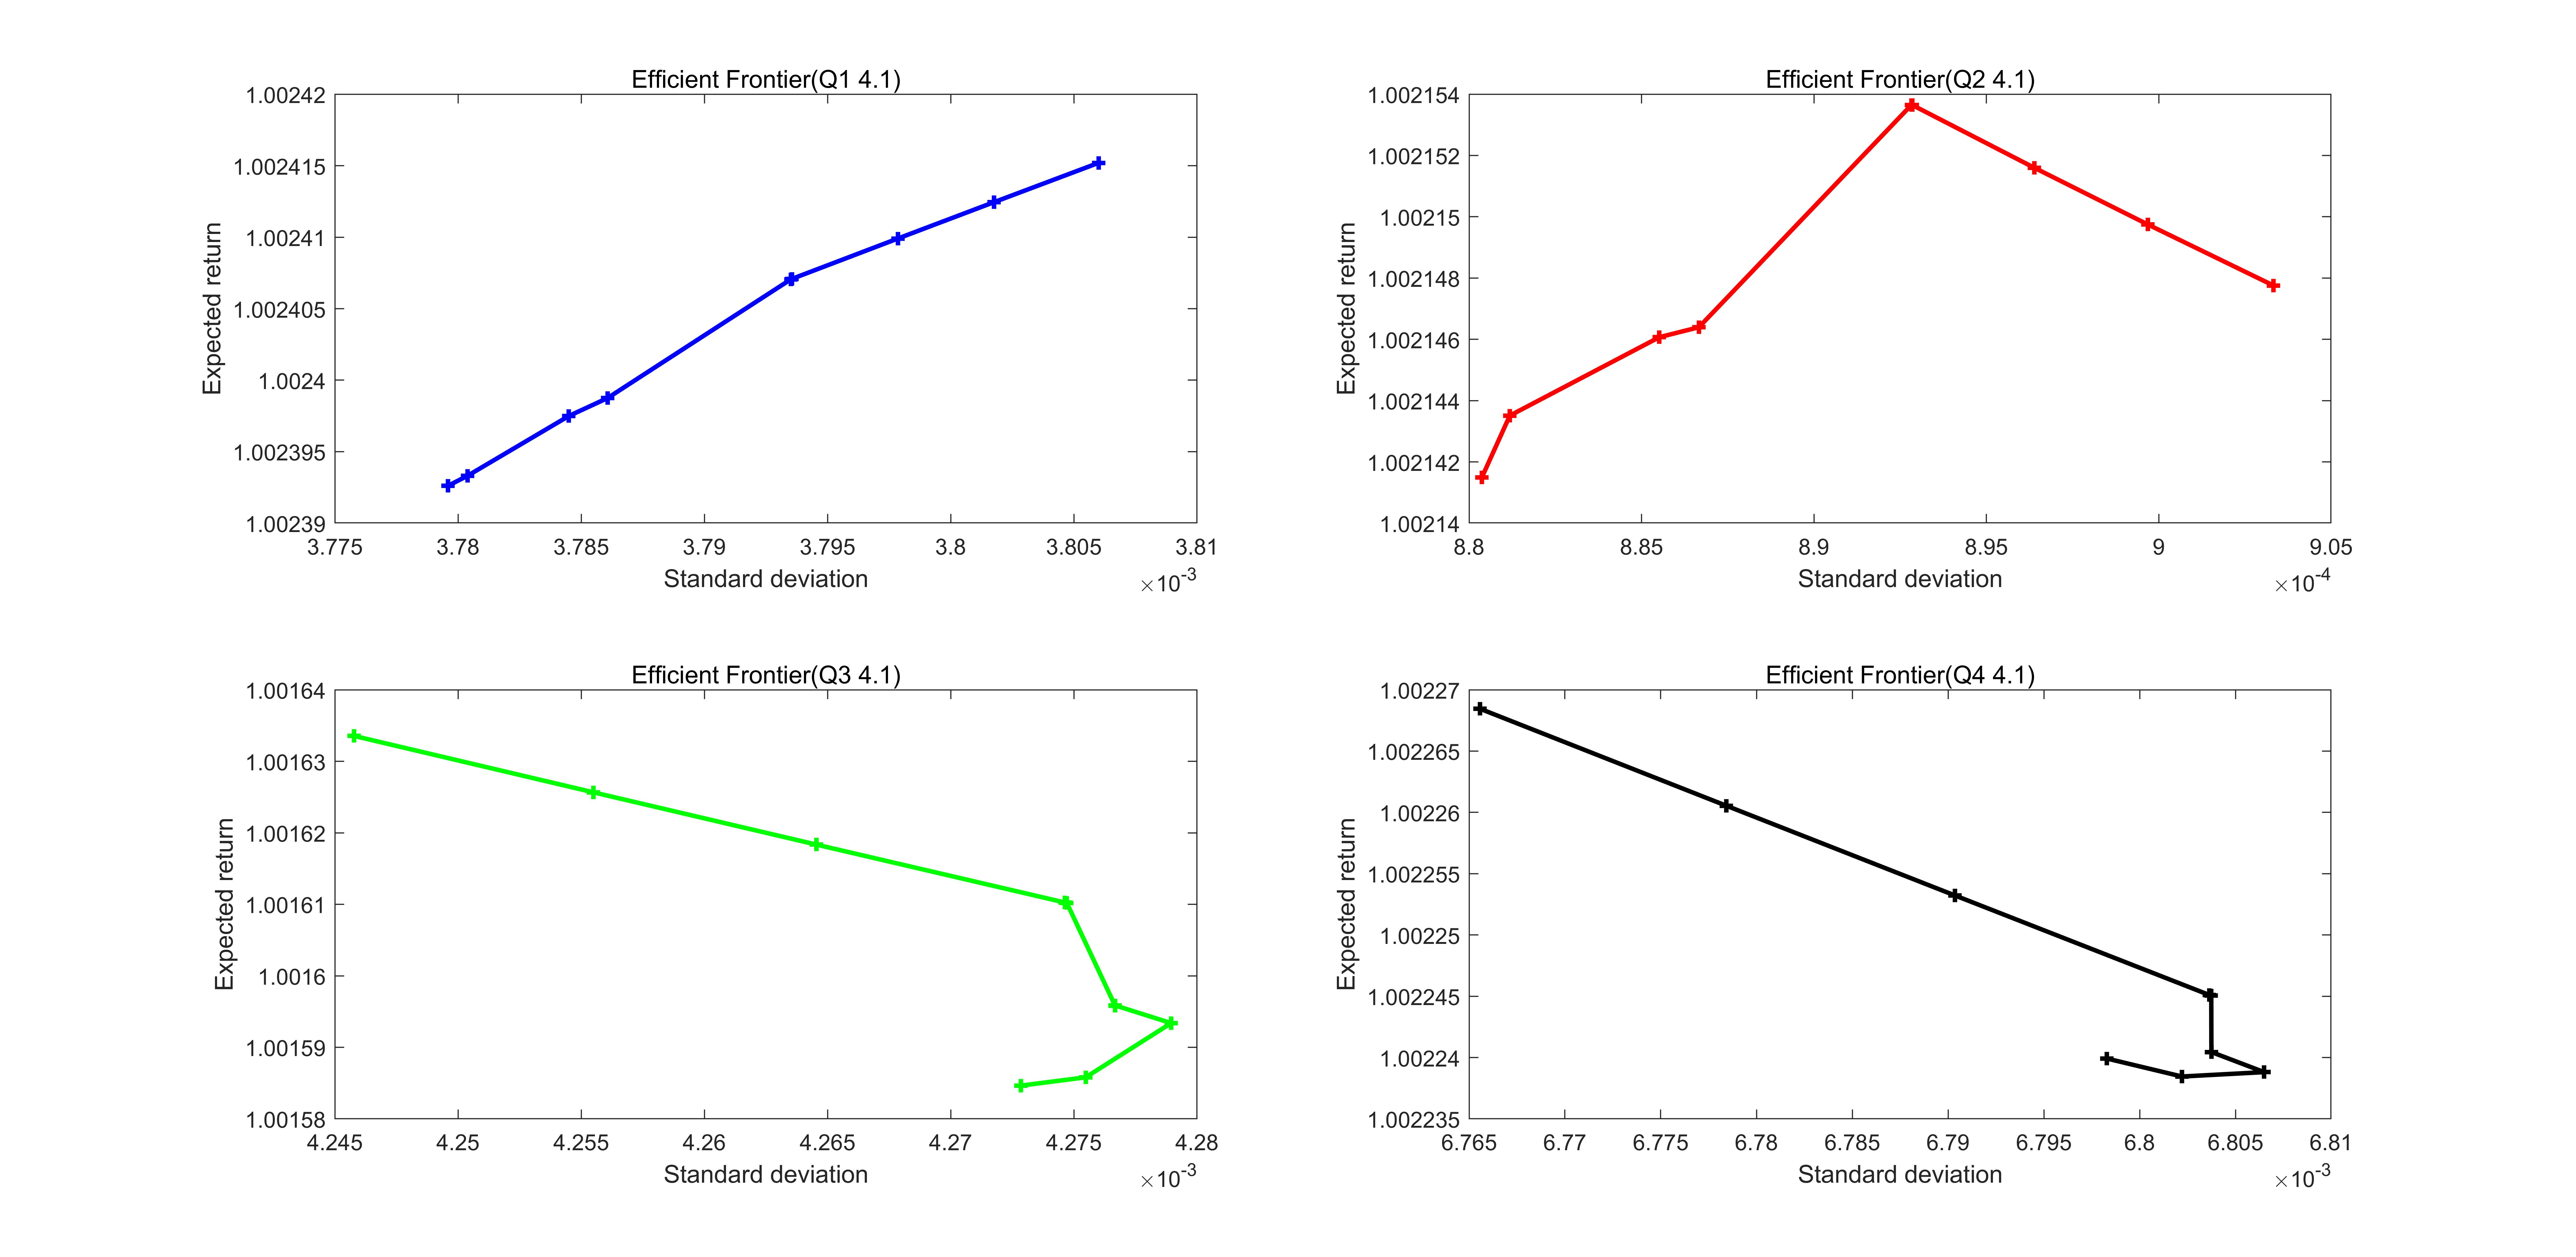
\includegraphics[width=1\textwidth]{41.jpg} %插入图片,[]中设置图片大小,{}中是图片文件名
	\caption{Efficient Frontier for Algorithm 1} 
	\label{Fig.main1} 
\end{figure}
\begin{figure}[H] 
	\centering 
	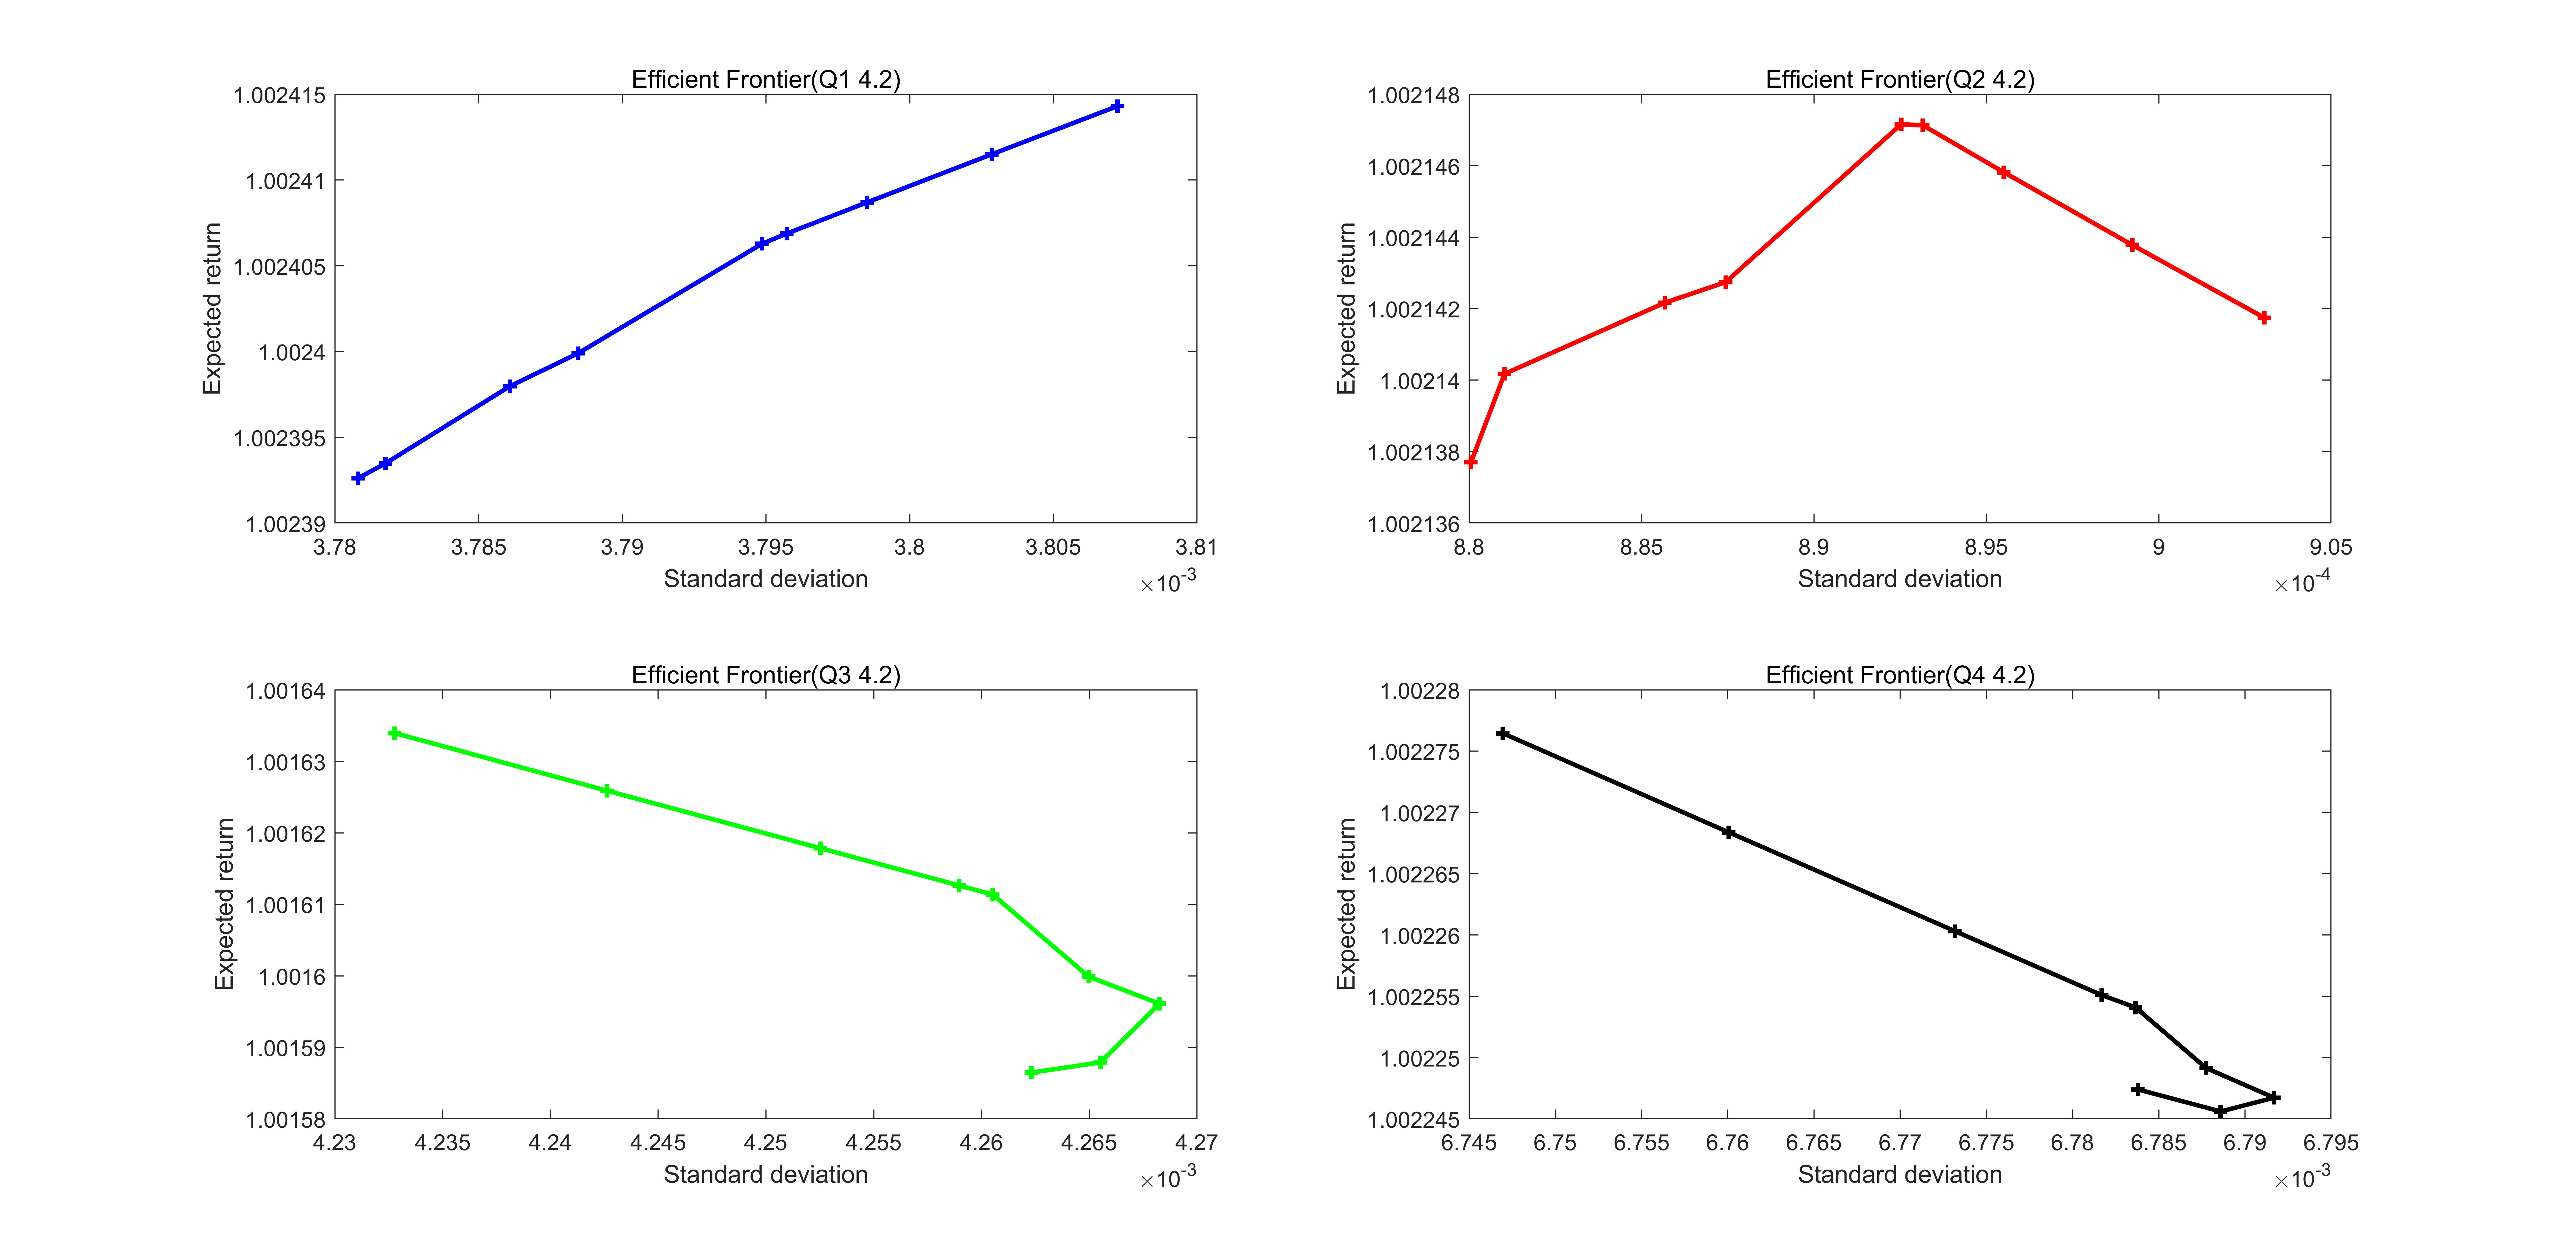
\includegraphics[width=1\textwidth]{42.jpg} %插入图片,[]中设置图片大小,{}中是图片文件名
	\caption{Efficient Frontier for Algorithm 2} 
	\label{Fig.main2} 
\end{figure}
\begin{figure}[H] 
	\centering 
	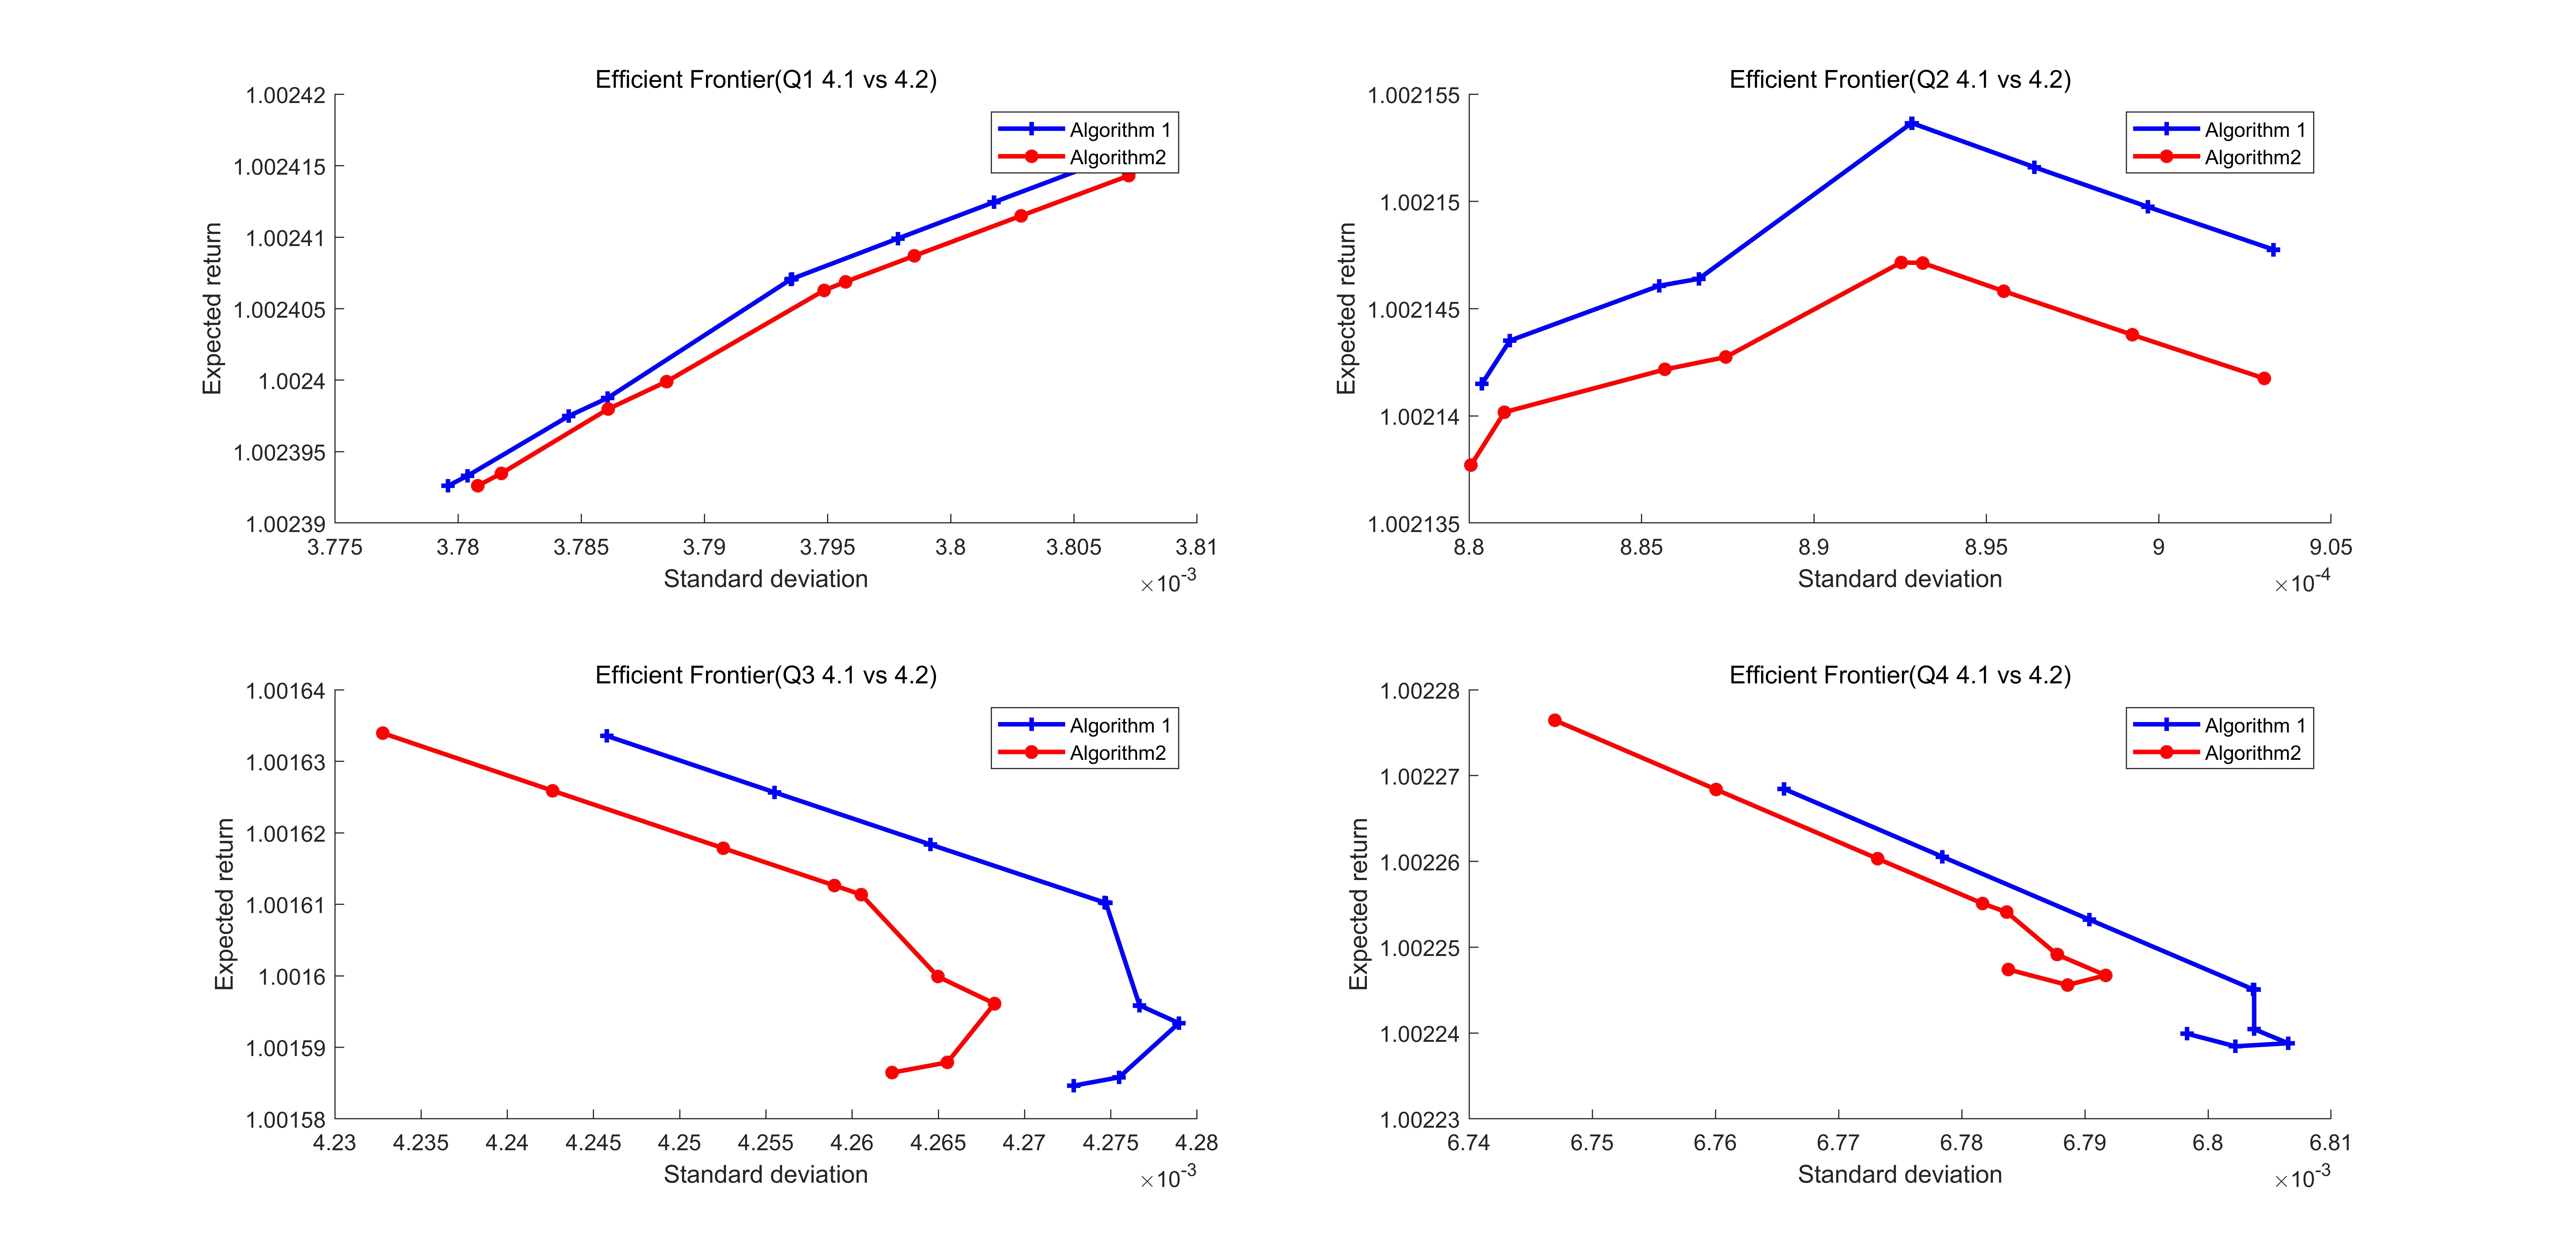
\includegraphics[width=1\textwidth]{412.jpg} %插入图片,[]中设置图片大小,{}中是图片文件名
	\caption{Efficient Frontier for Algorithm 1 \& 2} 
	\label{Fig.main3} 
\end{figure}
(5):
\begin{figure}[H] 
	\centering 
	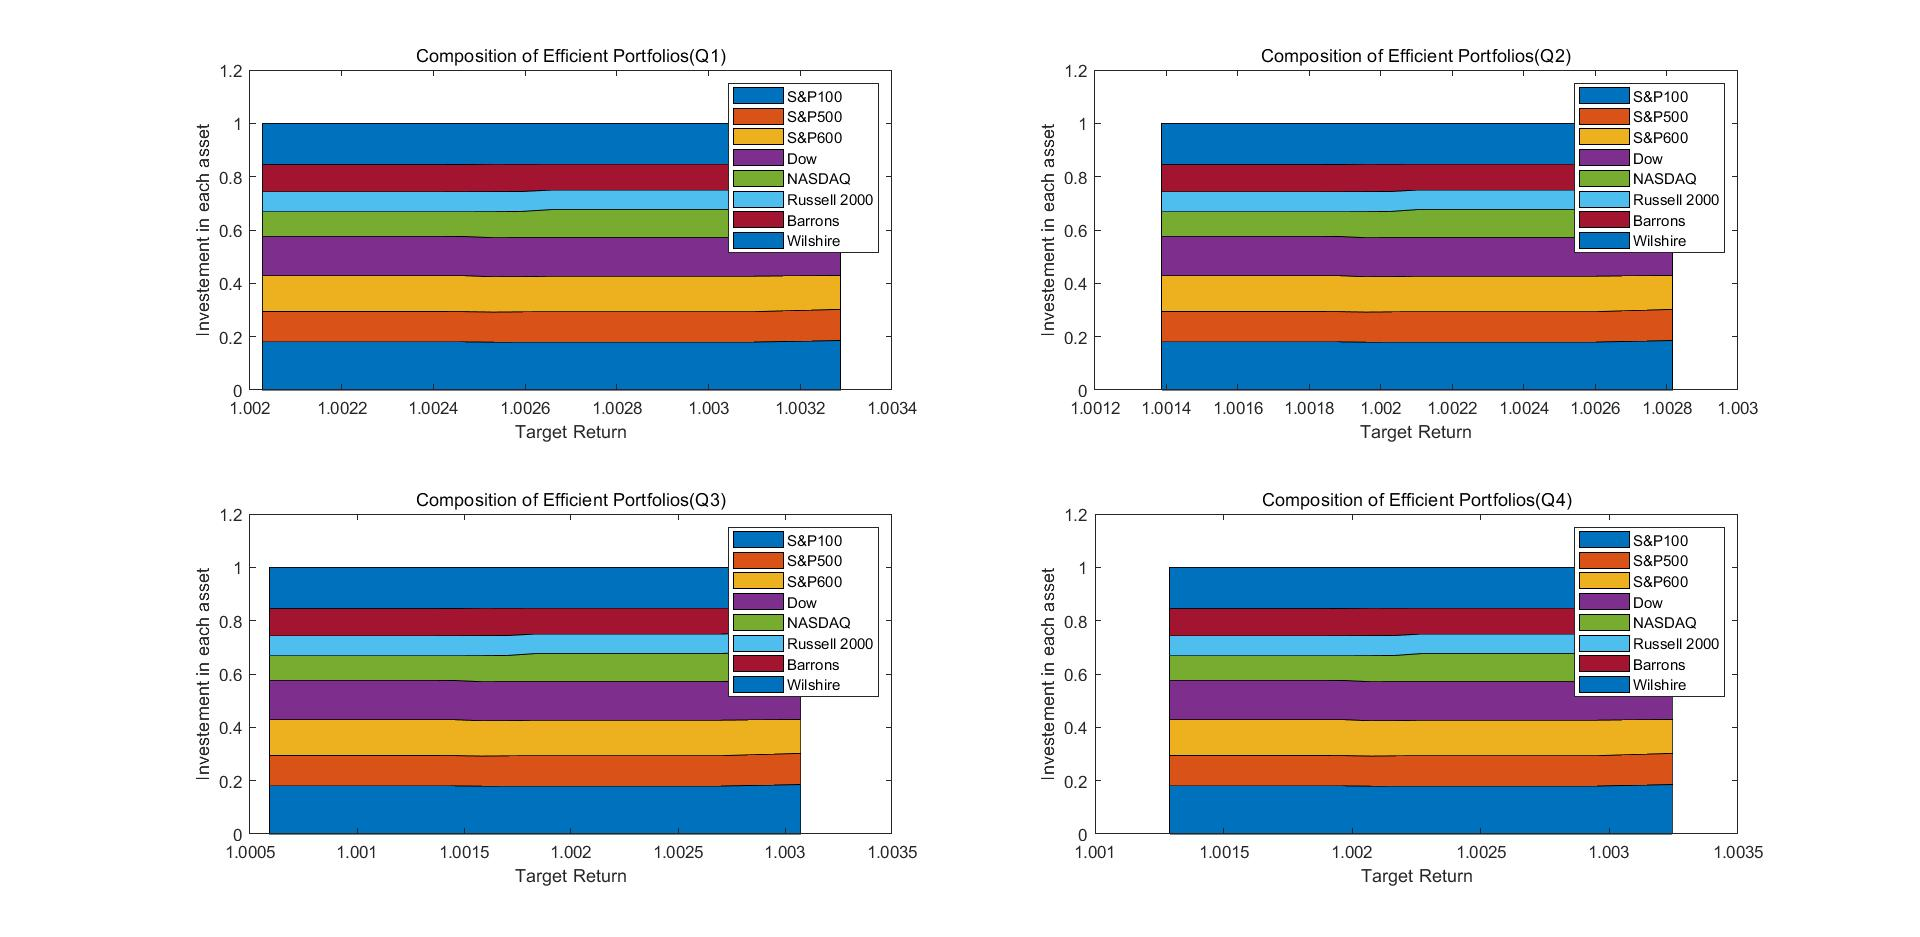
\includegraphics[width=1\textwidth]{51.jpg} %插入图片,[]中设置图片大小,{}中是图片文件名
	\caption{Composition of optimal portfolios, Algorithm 1, Target return} 
	\label{Fig.main4} 
\end{figure}
\begin{figure}[H] 
	\centering 
	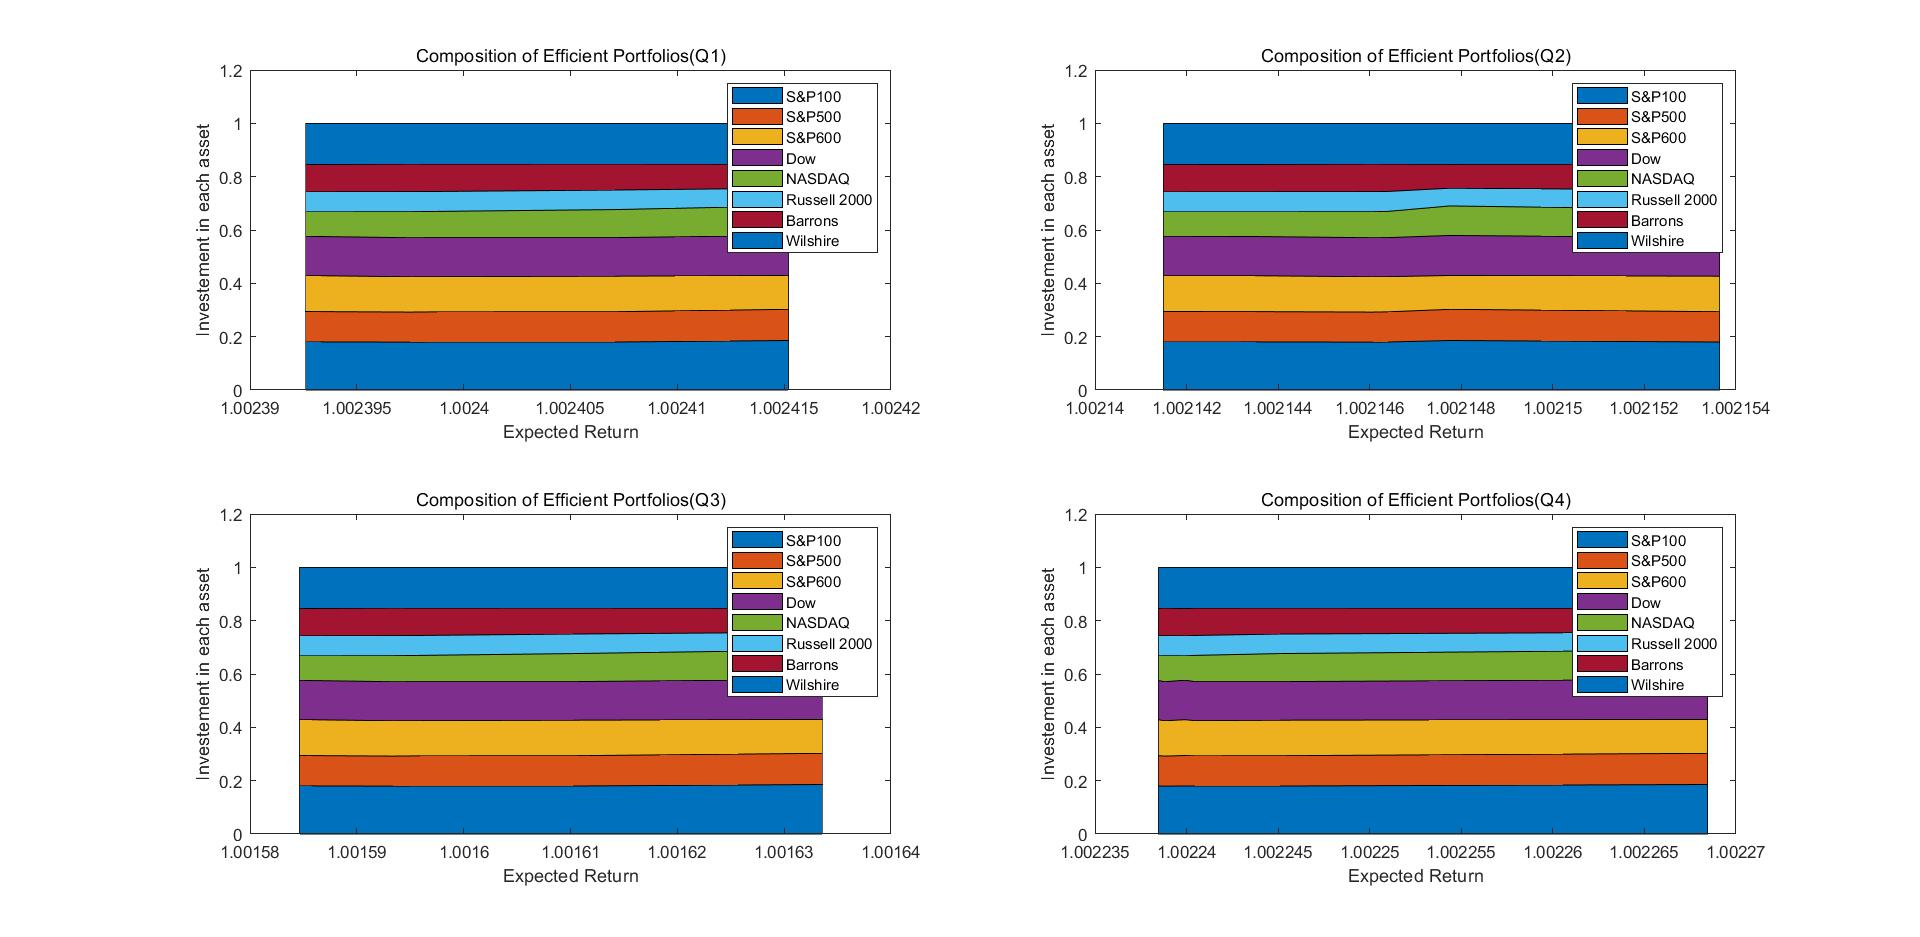
\includegraphics[width=1\textwidth]{52.jpg} %插入图片,[]中设置图片大小,{}中是图片文件名
	\caption{Composition of optimal portfolios, Algorithm 1, Expected return} 
	\label{Fig.main5} 
\end{figure}
\begin{figure}[H] 
	\centering 
	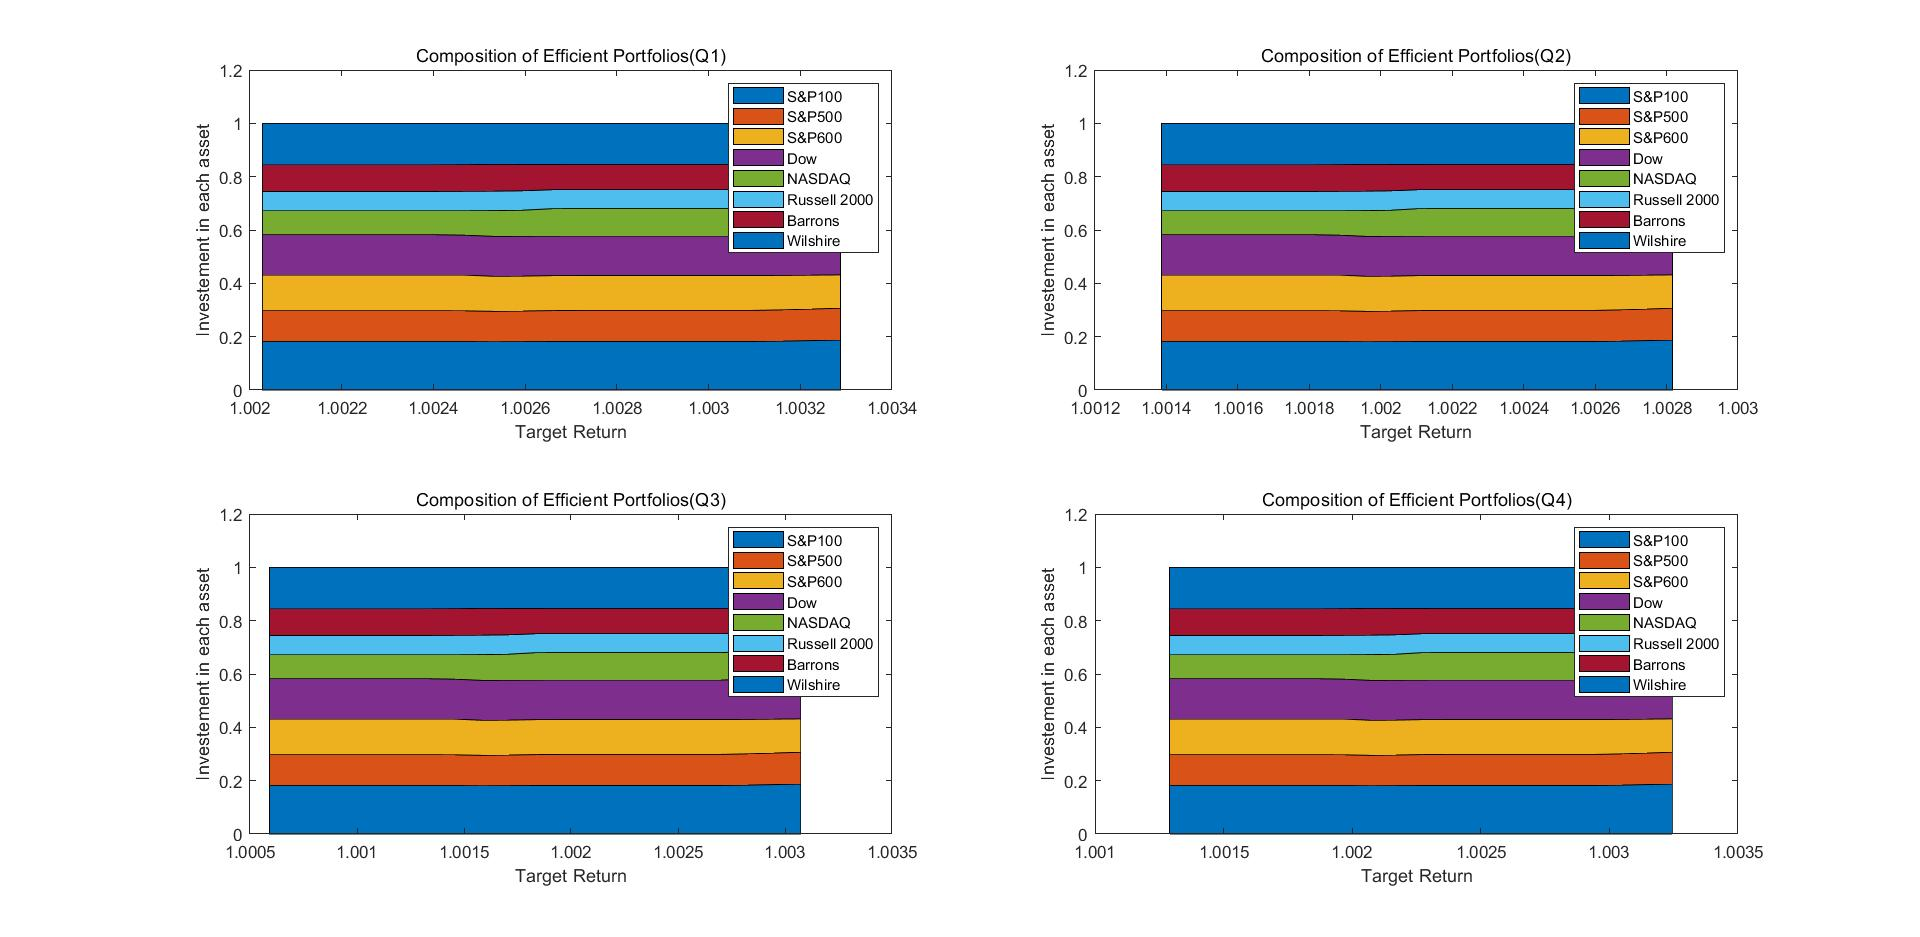
\includegraphics[width=1\textwidth]{53.jpg} %插入图片,[]中设置图片大小,{}中是图片文件名
	\caption{Composition of optimal portfolios, Algorithm 2, Target return} 
	\label{Fig.main6} 
\end{figure}
\begin{figure}[H] 
	\centering 
	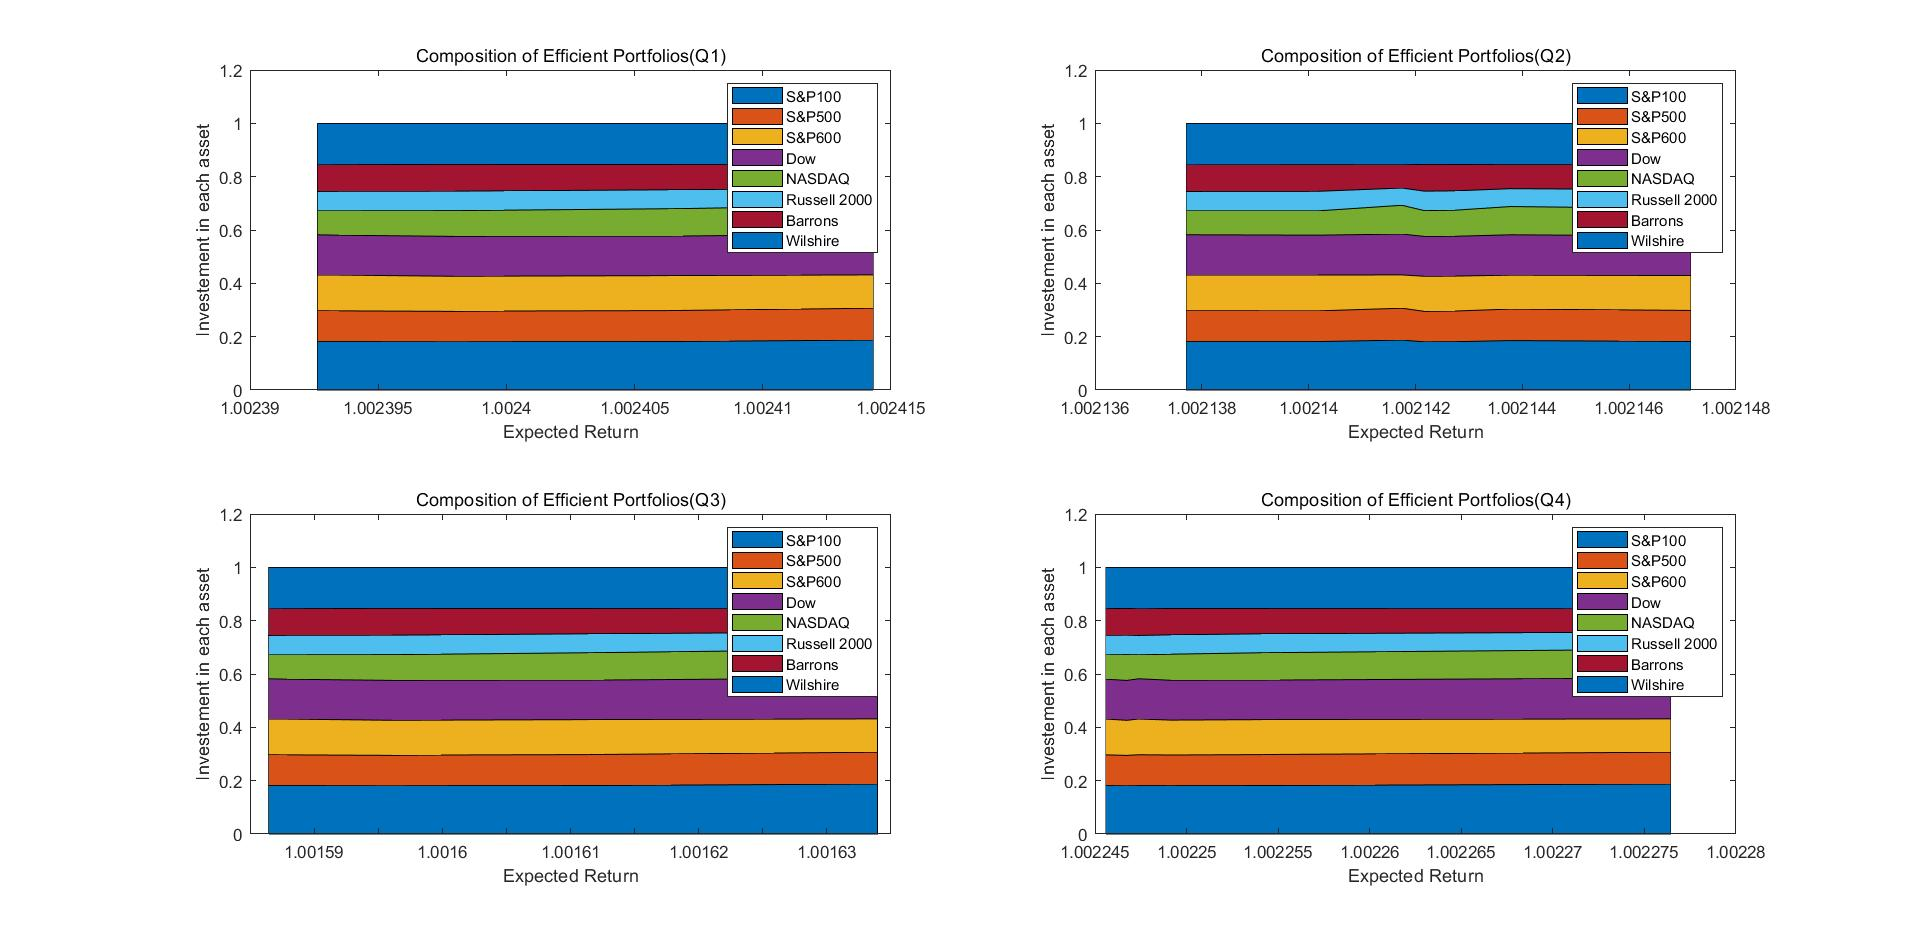
\includegraphics[width=1\textwidth]{54.jpg} %插入图片,[]中设置图片大小,{}中是图片文件名
	\caption{Composition of optimal portfolios, Algorithm 2, Expected return} 
	\label{Fig.main7} 
\end{figure}

\section*{Appendix}
\subsection*{Code of Question 3 (1)}
\begin{lstlisting}
import pandas as pd
import numpy as np
from scipy.stats.mstats import gmean

df = pd.DataFrame(pd.read_csv('indices2.csv'))
df_copy = pd.DataFrame(pd.read_csv('indices2.csv'))
Index = list(df.columns)
del Index[0]

# Question 1
# Calculate return rate
for j in Index:
for i in range(364):
df.loc[i+1,j]=df_copy.loc[i+1,j]/df_copy.loc[i,j]
df =df.drop(labels=0)
df.to_csv("df.csv", index_label="year")

# group by quarter
Q1 = df.loc[df['Date'].str.contains('Jan|Feb|Mar')]
Q2 = df.loc[df['Date'].str.contains('Apr|May|Jun')]
Q3 = df.loc[df['Date'].str.contains('Jul|Aug|Sep')]
Q4 = df.loc[df['Date'].str.contains('Oct|Nov|Dec')]

# Batch quarter
def get_return(datas):
rr = np.array([gmean(datas.loc[df['Date'].str.contains('2013')].iloc[:,1:])])
for year in range(2014,2020):
geometricMean = np.array([gmean(datas.loc[df['Date'].str.contains(f'{year}')].iloc[:,1:])])
rr = np.row_stack((rr,geometricMean))
return pd.DataFrame(data = rr,index = list(range(2013,2020)),columns=Index)

Q1_returnrates = get_return(Q1)
Q2_returnrates = get_return(Q2)
Q3_returnrates = get_return(Q3)
Q4_returnrates = get_return(Q4)

Q1_returnrates.to_csv("Q1_returnrates.csv", index_label="year")
Q2_returnrates.to_csv("Q2_returnrates.csv", index_label="year")
Q3_returnrates.to_csv("Q3_returnrates.csv", index_label="year")
Q4_returnrates.to_csv("Q4_returnrates.csv", index_label="year")

Q1.to_csv("Q1_raw.csv", index_label="year")
Q2.to_csv("Q2_raw.csv", index_label="year")
Q3.to_csv("Q3_raw.csv", index_label="year")
Q4.to_csv("Q4_raw.csv", index_label="year")
\end{lstlisting}
\subsection*{Code of Question 3 (2) \& (3)}
\begin{lstlisting}
clc
clear
% Question 3.1 & 3.2
Q1_returnrates = csvread('Q1_returnrates.csv',1,1);
Q2_returnrates = csvread('Q2_returnrates.csv',1,1);
Q3_returnrates = csvread('Q3_returnrates.csv',1,1);
Q4_returnrates = csvread('Q4_returnrates.csv',1,1);
mu_1 = geo_mean(Q1_returnrates);
mu_2 = geo_mean(Q2_returnrates);
mu_3 = geo_mean(Q3_returnrates);
mu_4 = geo_mean(Q4_returnrates);
Sigma_1 = cov(Q1_returnrates)*6/7;
Sigma_2 = cov(Q2_returnrates)*6/7;
Sigma_3 = cov(Q3_returnrates)*6/7;
Sigma_4 = cov(Q4_returnrates)*6/7;
% Generate target return rates.
% Question 3.3
R_1 = [];
R_2 = [];
R_3 = [];
R_4 = [];
for delta = 0:0.05:1
r_1 = min(mu_1) + delta * (max(mu_1) - min(mu_1));
r_2 = min(mu_2) + delta * (max(mu_2) - min(mu_2));
r_3 = min(mu_3) + delta * (max(mu_3) - min(mu_3));
r_4 = min(mu_4) + delta * (max(mu_4) - min(mu_4));
R_1 = [R_1 r_1];
R_2 = [R_2 r_2];
R_3 = [R_3 r_3];
R_4 = [R_4 r_4];
end

costs = [1.3 2.5 1.75 3.25];
returnrates = {Q1_returnrates,Q2_returnrates,Q3_returnrates,Q4_returnrates};
R = {R_1,R_2,R_3,R_4};
c = [0.45 1.15 0.65 0.8 1.25 1.1 0.9 0.7]*0.01;
\end{lstlisting}
\section*{Code of Question 4 (1)}
\begin{lstlisting}
% step 1
portfolio = 0.125 * ones(1,8);
x = 0.125 * ones(1,8);
for k = 0 : 10000
scenario = mod(k,7) + 1;
% step 2 Solve Q(x,w)
u = [0 0 0 0];
for t = 1 : 4
if (R{t}(11) - returnrates{t}(scenario,:) * x') > 0
u(t) = costs(t);
else
u(t) = 0;
end
end
P = zeros(1,8);
for i = 1 : 8
P(i) = -[returnrates{1}(scenario,i) returnrates{2}(scenario,i) returnrates{3}(scenario,i) returnrates{4}(scenario,i)] * u';
end
g = P;
% step 3 update x
x_new = projunitsimplex(x' - 1/(k + 1) * (c' + g'));
x = x_new';
portfolio = [portfolio ; x];
if k > 1
if max([norm(portfolio(k+2,:) - portfolio(k+1,:)), norm(portfolio(k+2,:) - portfolio(k,:)), norm(portfolio(k+2,:) - portfolio(k-1,:))]) < 1.0000e-06
break
end
end
end
\end{lstlisting}
\section*{Code of Question 4 (2)}
\begin{lstlisting}
% step 1 
portfolio = 0.125 * ones(1,8);
x = 0.125 * ones(1,8);
N = 7;
for k = 0 : 10000
% step 2 Solve Q(x,w)
gradient = zeros(1,8);
for scenario = 1 : N
y = [0 0 0 0];
y(1) = max([0, R{1}(11)-returnrates{1}(scenario,:)*x']);
y(2) = max([0, R{2}(11)-returnrates{2}(scenario,:)*x']);
y(3) = max([0, R{3}(11)-returnrates{3}(scenario,:)*x']);
y(4) = max([0, R{4}(11)-returnrates{4}(scenario,:)*x']);
R_matrix = [returnrates{1}(scenario,:) ; returnrates{2}(scenario,:) ; returnrates{3}(scenario,:) ; returnrates{4}(scenario,:)];
gradient = gradient + (-costs.*sign(y) * R_matrix);
end
g = 1 / N * gradient;
% step 3 update x
x_new = projunitsimplex(x' - 1/(k + 1) * (c' + g'));
x = x_new';
portfolio = [portfolio ; x];
if k > 1
if max([norm(portfolio(k+2,:) - portfolio(k+1,:)) norm(portfolio(k+2,:) - portfolio(k,:)) norm(portfolio(k+2,:) - portfolio(k-1,:))]) < 1.0000e-06
break
end
end
end
\end{lstlisting}
\section*{Code of Question 4 (3)}
\begin{lstlisting}
x_1 = [0.1799 0.1136 0.1332 0.1447 0.1052 0.0733 0.0976 0.1525];
x_2 = [0.1817 0.1160 0.1311 0.1483 0.1025 0.0710 0.0948 0.1545];
Q_1 = [];
Q_2 = [];
for scenario = 1 : 7
y_1 = [0 0 0 0];
y_2 = [0 0 0 0];
y_1(1) = max([0, R{1}(11)-returnrates{1}(scenario,:)*x_1']);
y_1(2) = max([0, R{2}(11)-returnrates{2}(scenario,:)*x_1']);
y_1(3) = max([0, R{3}(11)-returnrates{3}(scenario,:)*x_1']);
y_1(4) = max([0, R{4}(11)-returnrates{4}(scenario,:)*x_1']);
y_2(1) = max([0, R{1}(11)-returnrates{1}(scenario,:)*x_2']);
y_2(2) = max([0, R{2}(11)-returnrates{2}(scenario,:)*x_2']);
y_2(3) = max([0, R{3}(11)-returnrates{3}(scenario,:)*x_2']);
y_2(4) = max([0, R{4}(11)-returnrates{4}(scenario,:)*x_2']);
Q_1 = [Q_1 costs * y_1'];
Q_2 = [Q_2 costs * y_2'];
end
z_insample_1 = c * x_1' + sum(1/7 * Q_1);
z_insample_2 = c * x_2' + sum(1/7 * Q_2);

% out of sample
Q1_raw = csvread('Q1_raw.csv',1,2);
Q2_raw = csvread('Q2_raw.csv',1,2);
Q3_raw = csvread('Q3_raw.csv',1,2);
Q4_raw = csvread('Q4_raw.csv',1,2);
Q_raw = {Q1_raw Q2_raw Q3_raw Q4_raw};
outsample_scenario = min([size(Q1_raw,1) size(Q2_raw,1) size(Q3_raw,1) size(Q4_raw,1)]);
Q_1_outofsample = [];
Q_2_outofsample = [];
for scenario = 1 : outsample_scenario
y_1_outofsample = [0 0 0 0];
y_2_outofsample = [0 0 0 0];
y_1_outofsample(1) = max([0, R{1}(11)-Q_raw{1}(scenario,:)*x_1']);
y_1_outofsample(2) = max([0, R{2}(11)-Q_raw{2}(scenario,:)*x_1']);
y_1_outofsample(3) = max([0, R{3}(11)-Q_raw{3}(scenario,:)*x_1']);
y_1_outofsample(4) = max([0, R{4}(11)-Q_raw{4}(scenario,:)*x_1']);
y_2_outofsample(1) = max([0, R{1}(11)-Q_raw{1}(scenario,:)*x_2']);
y_2_outofsample(2) = max([0, R{2}(11)-Q_raw{2}(scenario,:)*x_2']);
y_2_outofsample(3) = max([0, R{3}(11)-Q_raw{3}(scenario,:)*x_2']);
y_2_outofsample(4) = max([0, R{4}(11)-Q_raw{4}(scenario,:)*x_2']);
Q_1_outofsample = [Q_1_outofsample costs * y_1_outofsample'];
Q_2_outofsample = [Q_2_outofsample costs * y_2_outofsample'];
end
z_outofsample_1 = c * x_1' + sum(1/outsample_scenario * Q_1_outofsample);
z_outofsample_2 = c * x_2' + sum(1/outsample_scenario * Q_2_outofsample);
\end{lstlisting}

\section*{Code of Question 4 (4)}
\subsection*{Algrithm 1}
\begin{lstlisting}
% Algorithm 1
opt_1 = [];
Q1_expected = [];
Q2_expected = [];
Q3_expected = [];
Q4_expected = [];
Q1_std = [];
Q2_std = [];
Q3_std = [];
Q4_std = [];
for target = 1 : 21
portfolio = 0.125 * ones(1,8);
x = 0.125 * ones(1,8);
for k = 0 : 10000
scenario = mod(k,7) + 1;
u = [0 0 0 0];
for t = 1 : 4
if (R{t}(target) - returnrates{t}(scenario,:) * x') > 0
u(t) = costs(t);
else
u(t) = 0;
end
end
P = zeros(1,8);
for i = 1 : 8
P(i) = -[returnrates{1}(scenario,i) returnrates{2}(scenario,i) returnrates{3}(scenario,i) returnrates{4}(scenario,i)] * u';
end
g = P;
x_new = projunitsimplex(x' - 1/(k + 1) * (c' + g'));
x = x_new';
portfolio = [portfolio ; x];
if k > 1
if max([norm(portfolio(k+2,:) - portfolio(k+1,:)) norm(portfolio(k+2,:) - portfolio(k,:)) norm(portfolio(k+2,:) - portfolio(k-1,:))]) < 1.0000e-06
break
end
end
end
opt_1 = [opt_1 x_new];
Q1_expected = [Q1_expected mu_1 * x_new];
Q2_expected = [Q2_expected mu_2 * x_new];
Q3_expected = [Q3_expected mu_3 * x_new];
Q4_expected = [Q4_expected mu_4 * x_new];
Q1_std = [Q1_std sqrt(x_new'*Sigma_1*x_new)];
Q2_std = [Q2_std sqrt(x_new'*Sigma_2*x_new)];
Q3_std = [Q3_std sqrt(x_new'*Sigma_3*x_new)];
Q4_std = [Q4_std sqrt(x_new'*Sigma_4*x_new)];
end


subplot(2,2,1)
plot(Q1_std,Q1_expected,'b+-','LineWidth',2);
title('Efficient Frontier(Q1 4.1)');
xlabel('Standard deviation');
ylabel('Expected return');

subplot(2,2,2)
plot(Q2_std,Q2_expected,'r+-','LineWidth',2);
title('Efficient Frontier(Q2 4.1)');
xlabel('Standard deviation');
ylabel('Expected return');

subplot(2,2,3)
plot(Q3_std,Q3_expected,'g+-','LineWidth',2);
title('Efficient Frontier(Q3 4.1)');
xlabel('Standard deviation');
ylabel('Expected return');

subplot(2,2,4)
plot(Q4_std,Q4_expected,'k+-','LineWidth',2);
title('Efficient Frontier(Q4 4.1)');
xlabel('Standard deviation');
ylabel('Expected return');

Q1_expected_alg1 = Q1_expected;
Q1_std_alg1 = Q1_std;

Q2_expected_alg1 = Q2_expected;
Q2_std_alg1 = Q2_std;

Q3_expected_alg1 = Q3_expected;
Q3_std_alg1 = Q3_std;

Q4_expected_alg1 = Q4_expected;
Q4_std_alg1 = Q4_std;
\end{lstlisting}
\subsection*{Algrithm 2}
\begin{lstlisting}
% Algorithm 2
opt_2 = [];
Q1_expected = [];
Q2_expected = [];
Q3_expected = [];
Q4_expected = [];
Q1_std = [];
Q2_std = [];
Q3_std = [];
Q4_std = [];
N = 7;
for target = 1 : 21
portfolio = 0.125 * ones(1,8);
x = 0.125 * ones(1,8);
for k = 0 : 10000
gradient = zeros(1,8);
for scenario = 1 : N
y = [0 0 0 0];
y(1) = max([0, R{1}(target)-returnrates{1}(scenario,:)*x']);
y(2) = max([0, R{2}(target)-returnrates{2}(scenario,:)*x']);
y(3) = max([0, R{3}(target)-returnrates{3}(scenario,:)*x']);
y(4) = max([0, R{4}(target)-returnrates{4}(scenario,:)*x']);
R_matrix = [returnrates{1}(scenario,:) ; returnrates{2}(scenario,:) ; returnrates{3}(scenario,:) ; returnrates{4}(scenario,:)];
gradient = gradient + (-costs.*sign(y) * R_matrix);
end
g = 1 / N * gradient;
x_new = projunitsimplex(x' - 1/(k + 1) * (c' + g'));
x = x_new';
portfolio = [portfolio ; x];
if k > 1
if max([norm(portfolio(k+2,:) - portfolio(k+1,:)) norm(portfolio(k+2,:) - portfolio(k,:)) norm(portfolio(k+2,:) - portfolio(k-1,:))]) < 1.0000e-06
break
end
end
end
opt_2 = [opt_2 x_new];
Q1_expected = [Q1_expected mu_1 * x_new];
Q2_expected = [Q2_expected mu_2 * x_new];
Q3_expected = [Q3_expected mu_3 * x_new];
Q4_expected = [Q4_expected mu_4 * x_new];
Q1_std = [Q1_std sqrt(x_new'*Sigma_1*x_new)];
Q2_std = [Q2_std sqrt(x_new'*Sigma_2*x_new)];
Q3_std = [Q3_std sqrt(x_new'*Sigma_3*x_new)];
Q4_std = [Q4_std sqrt(x_new'*Sigma_4*x_new)];
end

subplot(2,2,1)
plot(Q1_std,Q1_expected,'b+-','LineWidth',2);
title('Efficient Frontier(Q1 4.2)');
xlabel('Standard deviation');
ylabel('Expected return');

subplot(2,2,2)
plot(Q2_std,Q2_expected,'r+-','LineWidth',2);
title('Efficient Frontier(Q2 4.2)');
xlabel('Standard deviation');
ylabel('Expected return');

subplot(2,2,3)
plot(Q3_std,Q3_expected,'g+-','LineWidth',2);
title('Efficient Frontier(Q3 4.2)');
xlabel('Standard deviation');
ylabel('Expected return');

subplot(2,2,4)
plot(Q4_std,Q4_expected,'k+-','LineWidth',2);
title('Efficient Frontier(Q4 4.2)');
xlabel('Standard deviation');
ylabel('Expected return');

Q1_expected_alg2 = Q1_expected;
Q1_std_alg2 = Q1_std;

Q2_expected_alg2 = Q2_expected;
Q2_std_alg2 = Q2_std;

Q3_expected_alg2 = Q3_expected;
Q3_std_alg2 = Q3_std;

Q4_expected_alg2 = Q4_expected;
Q4_std_alg2 = Q4_std;
\end{lstlisting}
\subsection*{Compare algorithm 1 \& 2}
\begin{lstlisting}
subplot(2,2,1)
hold on 
plot(Q1_std_alg1,Q1_expected_alg1,'b+-','LineWidth',2);
plot(Q1_std_alg2,Q1_expected_alg2,'r*-','LineWidth',2);
xlabel('Standard deviation');
ylabel('Expected return');
legend('Algorithm 1','Algorithm2')
title('Efficient Frontier(Q1 4.1 vs 4.2)');
hold off 

subplot(2,2,2)
hold on 
plot(Q2_std_alg1,Q2_expected_alg1,'b+-','LineWidth',2);
plot(Q2_std_alg2,Q2_expected_alg2,'r*-','LineWidth',2);
xlabel('Standard deviation');
ylabel('Expected return');
legend('Algorithm 1','Algorithm2')
title('Efficient Frontier(Q2 4.1 vs 4.2)');
hold off 

subplot(2,2,3)
hold on 
plot(Q3_std_alg1,Q3_expected_alg1,'b+-','LineWidth',2);
plot(Q3_std_alg2,Q3_expected_alg2,'r*-','LineWidth',2);
xlabel('Standard deviation');
ylabel('Expected return');
legend('Algorithm 1','Algorithm2')
title('Efficient Frontier(Q3 4.1 vs 4.2)');
hold off 

subplot(2,2,4)
hold on 
plot(Q4_std_alg1,Q4_expected_alg1,'b+-','LineWidth',2);
plot(Q4_std_alg2,Q4_expected_alg2,'r*-','LineWidth',2);
xlabel('Standard deviation');
ylabel('Expected return');
legend('Algorithm 1','Algorithm2')
title('Efficient Frontier(Q4 4.1 vs 4.2)');
hold off 
\end{lstlisting}
\section*{Code of Question 4 (5)}
\begin{lstlisting}
assets = {'S&P100', 'S&P500', 'S&P600', 'Dow', 'NASDAQ', 'Russell 2000', 'Barrons', 'Wilshire'};
% Algorithm 1
subplot(2,2,1)
area(R{1},opt_1')
title('Composition of Efficient Portfolios(Q1)');
xlabel('Target Return');
ylabel('Investement in each asset');
legend(assets);

subplot(2,2,2)
area(R{2},opt_1')
title('Composition of Efficient Portfolios(Q2)');
xlabel('Target Return');
ylabel('Investement in each asset');
legend(assets);

subplot(2,2,3)
area(R{3},opt_1')
title('Composition of Efficient Portfolios(Q3)');
xlabel('Target Return');
ylabel('Investement in each asset');
legend(assets);

subplot(2,2,4)
area(R{4},opt_1')
title('Composition of Efficient Portfolios(Q4)');
xlabel('Target Return');
ylabel('Investement in each asset');
legend(assets);
%--------------------------------------------------------------------------
subplot(2,2,1)
area(Q1_expected_alg1,opt_1')
title('Composition of Efficient Portfolios(Q1)');
xlabel('Expected Return');
ylabel('Investement in each asset');
legend(assets);

subplot(2,2,2)
area(Q2_expected_alg1,opt_1')
title('Composition of Efficient Portfolios(Q2)');
xlabel('Expected Return');
ylabel('Investement in each asset');
legend(assets);

subplot(2,2,3)
area(Q3_expected_alg1,opt_1')
title('Composition of Efficient Portfolios(Q3)');
xlabel('Expected Return');
ylabel('Investement in each asset');
legend(assets);

subplot(2,2,4)
area(Q4_expected_alg1,opt_1')
title('Composition of Efficient Portfolios(Q4)');
xlabel('Expected Return');
ylabel('Investement in each asset');
legend(assets);
%--------------------------------------------------------------------------
%Algorithm 2
subplot(2,2,1)
area(R{1},opt_2')
title('Composition of Efficient Portfolios(Q1)');
xlabel('Target Return');
ylabel('Investement in each asset');
legend(assets);

subplot(2,2,2)
area(R{2},opt_2')
title('Composition of Efficient Portfolios(Q2)');
xlabel('Target Return');
ylabel('Investement in each asset');
legend(assets);

subplot(2,2,3)
area(R{3},opt_2')
title('Composition of Efficient Portfolios(Q3)');
xlabel('Target Return');
ylabel('Investement in each asset');
legend(assets);

subplot(2,2,4)
area(R{4},opt_2')
title('Composition of Efficient Portfolios(Q4)');
xlabel('Target Return');
ylabel('Investement in each asset');
legend(assets);
%--------------------------------------------------------------------------
subplot(2,2,1)
area(Q1_expected_alg2,opt_2')
title('Composition of Efficient Portfolios(Q1)');
xlabel('Expected Return');
ylabel('Investement in each asset');
legend(assets);

subplot(2,2,2)
area(Q2_expected_alg2,opt_2')
title('Composition of Efficient Portfolios(Q2)');
xlabel('Expected Return');
ylabel('Investement in each asset');
legend(assets);

subplot(2,2,3)
area(Q3_expected_alg2,opt_2')
title('Composition of Efficient Portfolios(Q3)');
xlabel('Expected Return');
ylabel('Investement in each asset');
legend(assets);

subplot(2,2,4)
area(Q4_expected_alg2,opt_2')
title('Composition of Efficient Portfolios(Q4)');
xlabel('Expected Return');
ylabel('Investement in each asset');
legend(assets);
\end{lstlisting}
\end{document}